%File: formatting-instruction.tex
\documentclass[letterpaper]{article}
\usepackage{url,graphicx,xcolor}
\usepackage{times}
\usepackage{helvet}
\usepackage{courier}
\usepackage[guidelines]{faikrmod3}
% \usepackage[]{faikrmod3} % without guidelines
\frenchspacing
\setlength{\pdfpagewidth}{8.5in}
\setlength{\pdfpageheight}{11in}



% THE \pdfinfo /Title AND /Author ARE NOT NECESSARY, THEY ARE METADATA FOR THE FINAL PDF FILE
\pdfinfo{
/Title (Insert Your Title Here)
/Author (Put All Your Authors Here, Separated by Commas)}
\setcounter{secnumdepth}{0}  
 \begin{document}
% The file aaai.sty is the style file for AAAI Press 
% proceedings, working notes, and technical reports.
%
\title{Guidelines and template for FAIKR-Mod3 Project Reports}
\author{First Student, Second Student, Third Student\\
Master's Degree in Artificial Intelligence, University of Bologna\\
\{ name1.surname11, name2.surname22, name3.surname33 \}@studio.unibo.it
}
\maketitle


\attention{DO NOT MODIFY THIS TEMPLATE - EXCEPT, OF COURSE FOR TITLE AND AUTHORS. REMOVE THE \texttt{guidelines} OPTION FROM  \texttt{$\backslash$usepackage[guidelines]\{faikrmod3\}} IN THE \LaTeX\ SOURCE IN THE FINAL VERSION.}

\begin{abstract}
\begin{quote}

\explanation{
This mini-project aims to ... \\
We use ... \\
We found that ...
}

\end{quote}
\end{abstract}


\section{Introduction}
\subsection{Domain}
\explanation{
Introduce your work: what you are modeling, if you are drawing inspiration from an existing model, study, paper, textbook example, challenge, \dots.\\
%
Briefly provide whatever background information on the domain you think is necessary for the reader to understand the model and your design choices.
}

\attention{HERE AND EVERYWHERE ELSE: ALWAYS KEEP IN MIND THAT, CRUCIALLY, WHATEVER TEXT/CODE/FIGURES/IDEAS/... YOU TAKE FROM ELSEWHERE MUST BE CLEARLY IDENTIFIED AND PROPERLY REFERENCED IN THE REPORT.}

\subsection{Aim}
\explanation{
Explain the purpose of your project: what do you intend to observe/try/experience/\dots? \\
\begin{itemize}
    \item 
Example: the purpose of this project is to implement part of the Bayesian network described in \cite{10.1371/journal.pone.0220065} and experiment with concepts seen in class \\
%
\item Another example: our aim was to experiment the effect of discretization of continuous variables \\
%
\item Yet another example: we are interested in comparing the run-time and error of approximate inference under different conditions
%
\item One final example: we studied \textit{value of information}: something mentioned in class but not covered in this module, which sparked our interest.
\end{itemize}
}
\subsection{Method}
\explanation{
Describe the methodology you followed
\begin{itemize}
    \item 
Example: we used pgmpy library methods\footnote{This is just an example: indeed, it is NOT necessary to use pgmpy; the coding language doesn't have to be python either. Feel free to use whatever software framework suits your needs.} to implement our network and run queries. To understand if differences in models, queries, parameters or number of samples induced differences in accuracy, we varied evidence nodes, conditional probability distributions, inference method, ...
\end{itemize}
}

\subsection{Results}

\explanation{
In a few lines: what are the most noteworthy results you have observed or things you have learned/understood from this project? (only the highlights: there will be a dedicated paragraph for presenting results in the Analysis section)
}

\section{Model}

\explanation{
Insert a picture of your Bayesian network(s) (Figure~\ref{fig:network})
%
\begin{figure}
    \centering
    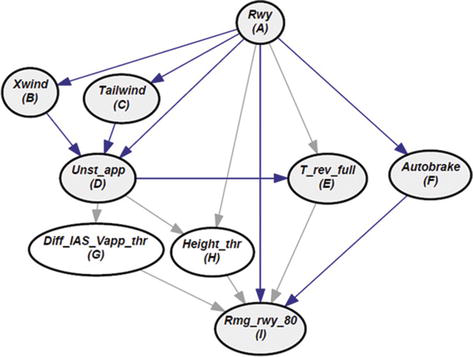
\includegraphics[scale=1.0]{F2.png}
    \caption{Bayesian network. Image taken from \url{https://www.intechopen.com/chapters/62844}}
    \label{fig:network}
\end{figure}
}

\explanation{
Explain the following aspects of your model (if there is too much to say and not enough space, put in your notebook whatever does not fit here):
\begin{itemize}
    \item nodes: if not self-explanatory, explain each random variable's meaning/intuition and type/range
    \item conditional distributions (for example, the CPTs, some or all of them)
    \item the procedure you followed to build your model (structure and conditional distributions): from reference paper? by analyzing the domain? learned from data? just assigned probability distributions arbitrarily? followed a particular methodology for building the network? ...
\end{itemize}  
In general, only write whatever is relevant and necessary to understand the rest of the report. Do not explain concepts seen in class or explained in textbooks. Do not describe models taken from textbook/literature/tutorials/libraries, like (for example) the Asia network. Instead, if you are using a model as-is: just insert a reference or URL\footnote{\url{https://www.bnlearn.com/bnrepository/}.}
}

\section{Analysis}

\subsection{Experimental setup}
\explanation{
Briefly describe the probability queries or other experiments that you have carried out. Describe how you plan to evaluate the results (for example: are there results that you would expect?)
}

\subsection{Results}
\explanation{
What did you observe? \\
%
All according to expectations? \\
%
Anything surprising or worthwhile mentioning?
}


\section{Conclusion}
\explanation{
Just one paragraph: what you have learned, anything interesting that came up, what are the limitations of your model/experiments/study/...
}


\section{Links to external resources}
\explanation{
Optionally, insert here:
\begin{itemize}
    \item a link to your GitHub or any other public repo where one can find your code (only if you did not submit your code on Virtuale) 
    \item a link to your dataset (only if you have used a dataset, for example, for learning network parameters or structure)
\end{itemize}
Leave this section empty if you have all your resources in Virtuale. \textbf{Do not insert code/outputs in this report}.
}
\bigskip

\bibliographystyle{aaai}
\bibliography{faikrmod3.bib}


\attention{NOTICE: THIS REPORT'S LENGTH MUST NOT EXCEED \textbf{TWO PAGES} PLUS REFERENCES. THIS MAY MEAN THAT YOU WILL HAVE TO LEAVE OUT OF THE REPORT PART OF THE WORK YOU HAVE DONE OR OBSERVATIONS YOU HAVE. THIS IS NORMAL: THE REPORT SHOULD EMPHASIZE WHAT IS MOST SIGNIFICANT, NOTEWORTHY, AND REFER TO THE NOTEBOOK FOR ANYTHING ELSE. FOR ANY OTHER ASPECT OF YOUR WORK THAT YOU WOULD LIKE TO EMPHASIZE BUT CANNOT EXPLAIN HERE FOR LACK OF SPACE, FEEL FREE TO ADD COMMENTS IN THE NOTEBOOK.}


\end{document}